\chapter{Охрана труда и безопасность в чрезвычайных ситуациях}

\section{Анализ условий труда на рабочем месте аналитика в НИЛ}

Производственное помещение, научно-исследовательская лаборатория (НИЛ), содержит
четыре рабочих мест, каждое из которых оборудовано ПК в комплекте: системный
блок, жидкокристаллический экран, компьютерная мышь, клавиатура.

Размеры помещения составляют 5x4,6x3 м. Нормой, в соответствии с ДСанПиН
3.3.2-007-98, является площадь на одно робочее место не менее 6,0 $\text{м}^2$
объём --- не менее 20,0 $\text{м}^3$. Помещение НИЛ включает 4 рабочих места
площадью 23 $\text{м}^2$ и объёмом 69 $\text{м}^3$, что составляет 5,75
$\text{м}^2$ площади и 17.25 $\text{м}^3$ объёмом на одно рабочее место, что не
соответствует требованиям ДСанПиН 3.3.2-007-98.

В помещении имеются два окна общей площадью 8 $\text{м}^2$.

С целью анализа условий труда в помещении НИЛ была рассмотрена система
''Человек-Машина-Среда'' (Ч-М-С).

Ч1-Ч4 --- коллектив людей, состоящий из 4 человека, работающих одновременно в
пределах одного помещения. Состоит из трех функциональных частей:

Чx.1 --- аналитик, который выполняет работу на ПК.

Чx.2 --- аналитик, который рассматривается с точки зрения влияния на окужающую
среду.

Чx.3 --- психофизиологическое состояние человека.

М1-М4 --- комплекс оборудования для осуществления трудового процесса (проведения
исследований). Представлен четырьмя ПК:

Мx.1 --- ПК, используемый аналитиком.

Мx.2 --- аварийная защита ПК.

Мx.3 --- влияние ПК на окружающую среду и человека.

Среда --- внутренняя среда помещения: освещение, микроклимат.

ПТ --- предмет труда --- исследование методов формирования узлов замен блочных
симметричных шифров.

Структура системы Ч-М-С рассмотрена на рисунке~\ref{fig:worker_safety_hme}.
Направление и содержание связей сведены в таблицу~\ref{table:worker_safety_HME}

\begin{figure}
    \begin{center}
       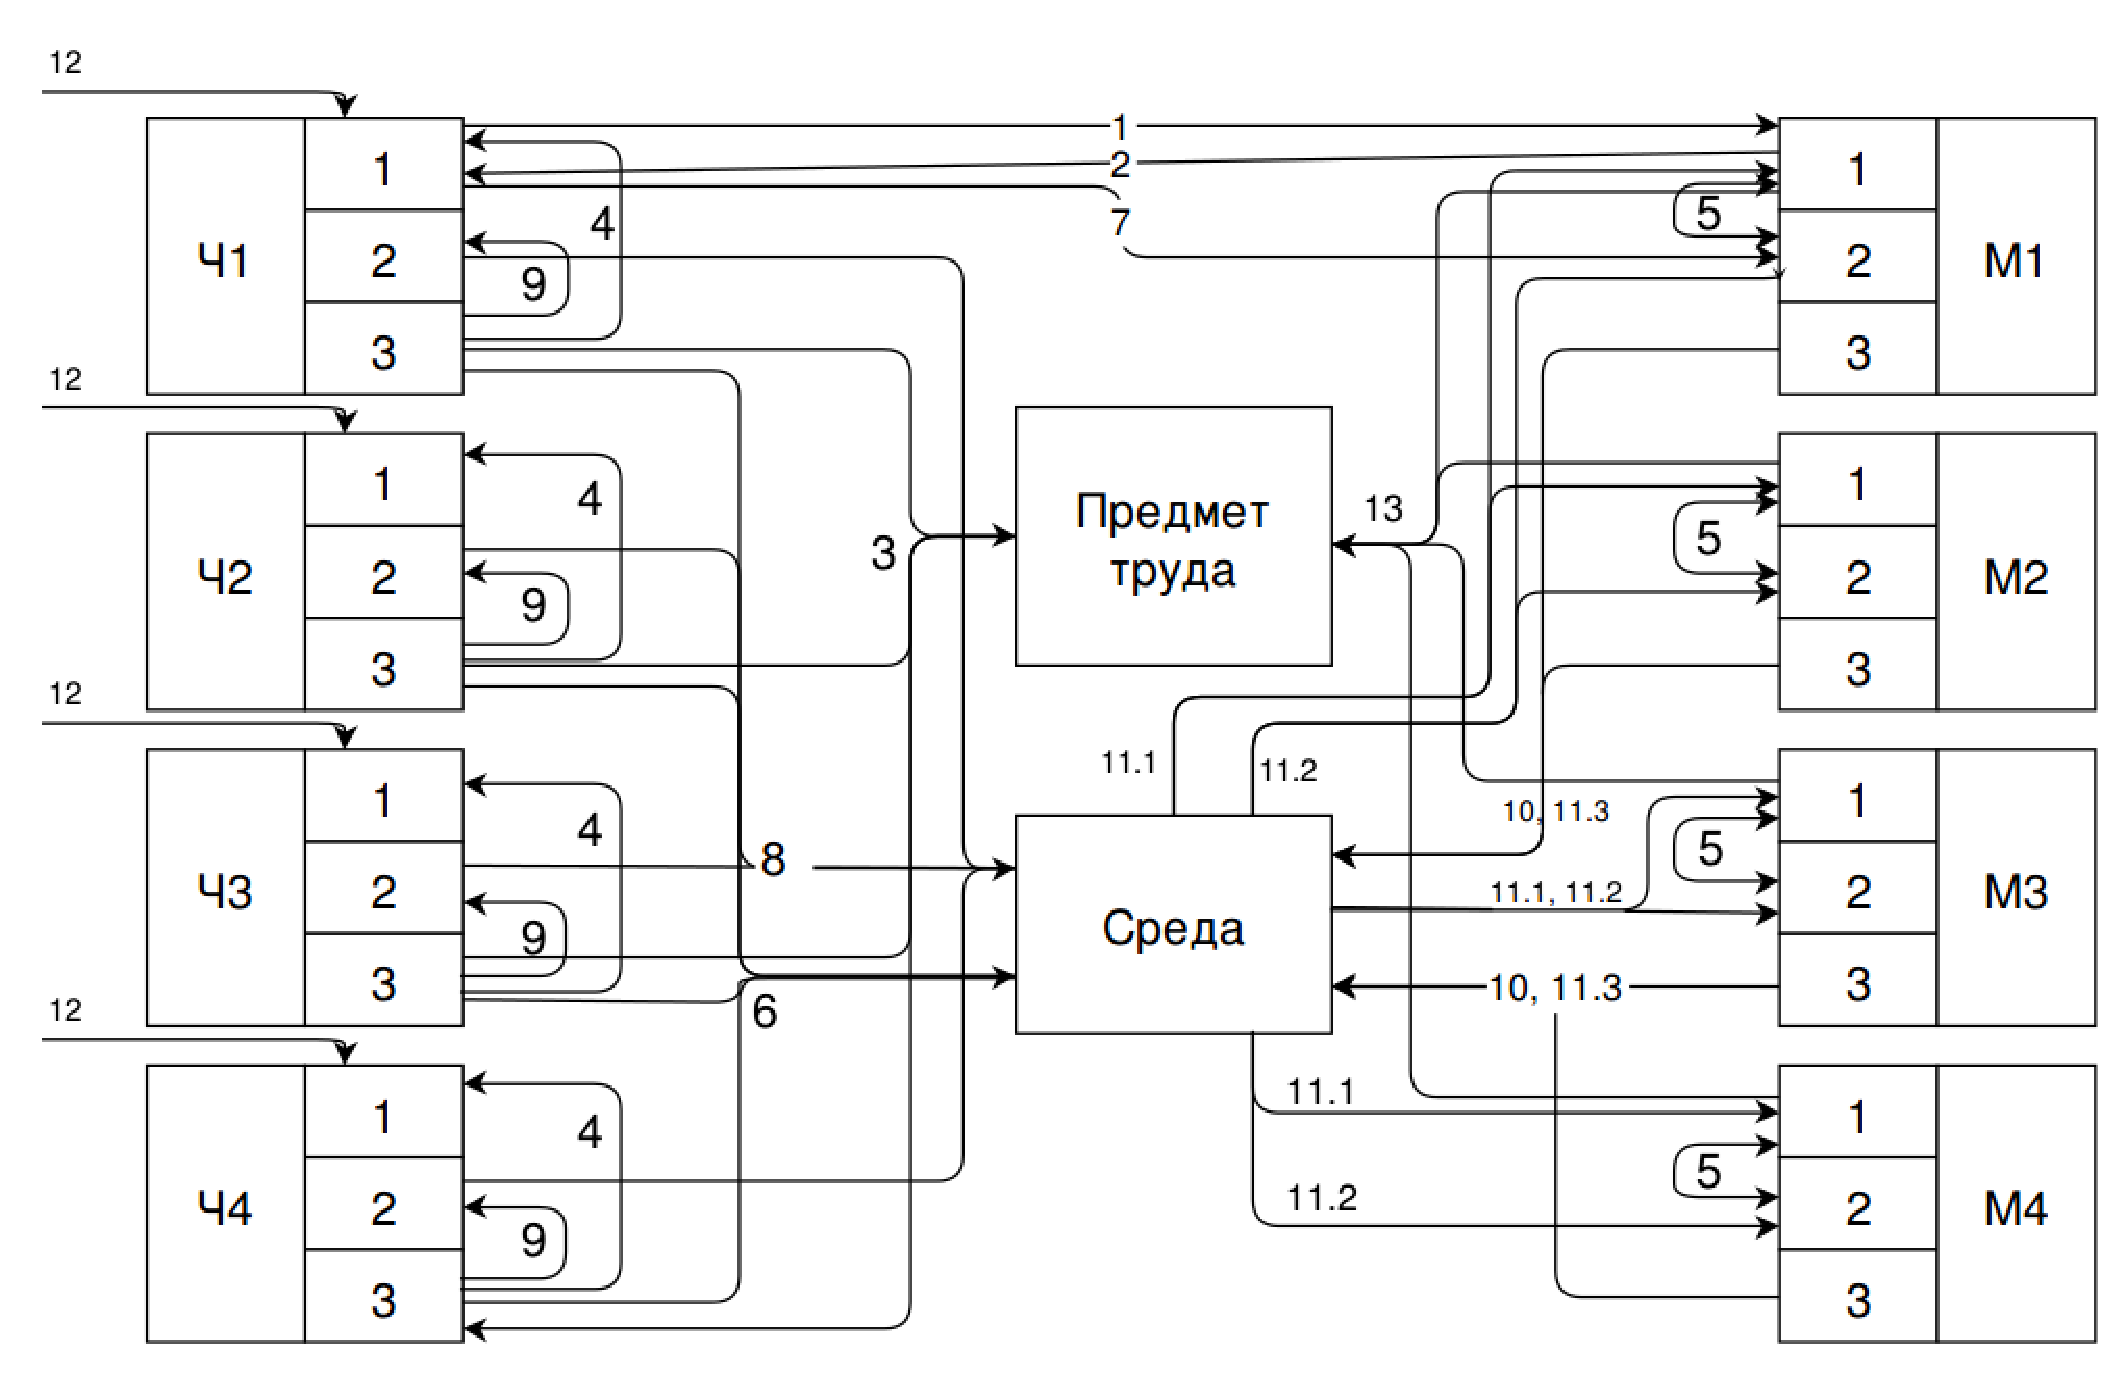
\includegraphics[width=1\textwidth]{graphics/worker_safety_hme.eps}
    \end{center}
    \caption{Cтруктура системы Ч-М-С}
    \label{fig:worker_safety_hme}
\end{figure}

\begin{table}
    \caption{Декомпозиция системы Ч-М-С.}
    \label{table:worker_safety_HME}
    \def\arraystretch{1.25}
    \begin{tabular}{| m{1.3cm} | m{2.3cm} | m{11.7cm} |}
        \hline
        Номер связи & Направ- ления связи   & Содержание связи                                                                                          \\ \hline
        1           & Чx.1-Мx.1             & Влияние человека на ПК и его настройки                                                                    \\ \hline
        2           & Мx.1-Чx.1             & Информация про состояние ПК                                                                               \\ \hline
        3           & ПТ-Чx.3               & Влияние процесса анализа атак на психологическое состояние аналитика                                      \\ \hline
        4           & Чx.3-Чx.1             & Уменьшение продуктивности работы вследствие монотонности труда и умственного перенапряжения               \\ \hline
        5.1         & Мx.1-Мx.2             & Информация, необходимая для генерации аварийного управляющего влияния                                     \\ \hline
        5.2         & Мx.2-Мx.1             & Недостаточная освещённость и вентиляция рабочего места                                                    \\ \hline
        6           & С-Чx.3                & Влияние среды на состояние организма аналитика                                                            \\ \hline
        7           & Чx.1-Мx.2             & Влияние аналитика на аварийное состояние ПК                                                               \\ \hline
        8           & Чx.2-С                & Выделения углекислого газа вследствие процесса дыхания, выделение тепла и пота                            \\ \hline
        9           & Чx.3-Чx.2             & Влияние психофизиологического состояния на степень интенсивности обмена веществ между организмом и средой \\ \hline
        10          & Мx.3-С                & Электромагнитные излучения, шум, температура                                                              \\ \hline
        11.1        & C-Мх.1                & \multirow{2}{*}{\vbox{Влияние параметров окружающей среды (температура, влажность, запылённость) на работу ПК}} \\ \cline{1-2}
        11.2        & С-Мх.2                & \\ \cline{1-2}
        11.3        & С-Мх.3                & \\ \hline
        12          & Внешняя система управления - Лх.1 & Информация про общий технологический процесс                                                    \\ \hline
        13          & Мх.1-ПТ               & Влияние машины на предмет труда. Непредвиденное отлючение питания, приводящее к остановке рабочего процесса \\ \hline
    \end{tabular}
\end{table}

Потенциально опасными и вредными производственнми факторами по ГОСТ 12.0.003-74
для данного помещения НИЛ являются:

\begin{enumerate}
    % fake second level of itemize
    \setitemize[1]{leftmargin=1.25cm,itemindent=2cm,listparindent=-2cm}

    \item физические:

    \begin{itemize}

        \item повышенная или пониженная температура воздуха рабочей зоны;
        
        \item повышенная или пониженная подвижность воздуха;
        
        \item отсутствие или недостаток естественного света;
        
        \item недостаточная освещённость рабочей зоны;
        
    \end{itemize}

    \item химические: отсутствуют;
   
    \item биологические: отсутствуют;
    
    \item психофизиологические:

    \begin{itemize}

        \item монотонность труда;

        \item умственное перенапряжение;

        \item перенапряжение анализаторов (зрительные).

    \end{itemize}

\end{enumerate}

Результаты оценки факторов производственной среды и трудового процесса приведены в табл.~\ref{table:evaluation_of}.

\begin{center}
    \fontsize{10pt}{8pt}\selectfont
    \def\arraystretch{1.55}
    \begin{longtable}{| >{\raggedright\arraybackslash}m{5cm} | >{\centering\arraybackslash}p{2.5cm} | >{\centering\arraybackslash}p{2.5cm} | >{\centering\arraybackslash}p{0.7cm} | >{\centering\arraybackslash}p{0.7cm} | >{\centering\arraybackslash}p{0.7cm} | >{\centering\arraybackslash}p{2cm} |}
        \caption{\label{table:evaluation_of}Оценка факторов производственной среды и трудового процесса} \\ \hline
        \multirow{2}{*}{\vbox{\centering{Факторы производственной среды и процесса труда}}} &
            \multicolumn{2}{m{5cm}}{\centering{Значение фактора (ПДК, ПДР)}} &
            \multicolumn{3}{|m{3cm}|}{\centering{3-й класс --- опасные и вредные условия, характер труда}} &
            \multirow{2}{*}{\vbox{\centering{Длительность действия фактора, в \% за смену}}} \\ \cline{2-6}
          & Норма & Факт & 1 ст. & 2 ст. & 3 ст. & \\ \hline
        \endfirsthead
        \multicolumn{7}{r}{\fontsize{14pt}{14pt}\selectfont Продолжение таблицы \thetable} \\ \hline
        \hline
        \centering{1} & 2 & 3 & 4 & 5 & 6 & 7 \\ \hline
        \hline
        \endhead
        \hline
        \endlastfoot
        \centering{1} & 2 & 3 & 4 & 5 & 6 & 7 \\ \hline
        1. Вредные хим. вещества: & & & & & & \\
           1-й класс опасности & - & - & - & - & - & -\\ \hline
           2-й класс опасности & - & - & - & - & - & -\\ \hline
           3-4-й класс опасности & - & - & - & - & - & -\\ \hline
        2. Вибрация & - & - & - & - & - & -\\ \hline
        3. Шум, дБ & До 50 & 49 & - & - & - & 93\\ \hline
        4. Инфразвук & - & - & - & - & - & -\\ \hline
        5. Ультразвук & - & - & - & - & - & -\\ \hline
        6. Неионизирующее излучение радиочастотного диапазона, В/м & 5~Гц .. 2~кГц -- 25; 2 кГц...400 кГц -- 2,5 & 5~Гц .. 2~кГц -- до~25; 2~кГц .. 400~кГц -- до 2,5 & - & - & - & 93\\ \hline
        7. Рентгеновское излучение, мкР/ч & До 100 & 14 & - & - & - & 100\\ \hline
        8. Микроклимат: & & & & & & \\ 
        \multirow{2}{*}{\vbox{8.1 Температура воздуха, С}} & х: 22-24 & 23 & - & - & - & 100\\
         & т: 23-25 & 24 & - & - & - & 100\\ \hline
        \multirow{2}{*}{\vbox{8.2 Скорость движения воздуха, м/с}} & х: 0,1 & менее 0,1 & - & - & - & 100\\ 
         & т: 0,1 & менее 0,1 & - & - & - & 100\\ \hline
        \multirow{2}{*}{\vbox{8.3 Относительная влажность, \%}} & х: 60-40 & 57 & - & - & - & 100\\ 
         & т: 60-40 & 52 & - & - & - & 100\\ \hline
        9. Атмосферное давление, мм. рт. ст. & 740-760 & 744 & - & - & - & 100\\ \hline
        10. Освещение: & & & & & & \\ 
        10.1 Естественное (КЕО) & 1,2 & 1,6 & - & - & - & 93\\ \hline
        10.2 Искусственное, лк & 300-500 & 370 & - & - & - & 93\\ \hline
        11. Тяжесть труда: & & & & & & \\ 
        11.1 Мелкие стереотипные движения кистей и пальцев рук & До 40000 & 20000 & - & - & - & 80\\ \hline
        11.2 Рабочая поза (нахождение в наклоненном положении в течение смены) & До 25\% времени за смену & Поза свободная & - & - & - & 93\\ \hline
        11.3 Наклоны корпуса тела (раз за смену) & 51-100 & Произвольные & - & - & - & 93\\ \hline
        11.4 Перемещения в пространстве (по горизонтали), км за смену & До 8 & 0,1 & - & - & - & 93\\ \hline
        Напряженность труда & & & & & & \\ 
        а) внимание & & & & & & \\ 
        - длительность сосредоточенного восприятия (\% от времени смены & 25-50 & 48 & - & - & - & 93\\ \hline
        - плотность сигналов (световых, звуковых) и сообщений, за час & 75-175 & 250 &  & + &  & 93\\ \hline
        б) нагрузка на анализаторы & & & & & & \\ 
        - зрительный, наблюдение за экранами ВДТ, ч за смену & 2-3 & 3 & - & - & - & 93\\ \hline
        - слуховой, восприятие речи или сигналов & Разборчивость слов и сигналов от 90\% до 70\% от их кол-ва & 99\% разборчивых слов и сигналов & - & - & - & 93\\ \hline
        в) монотонность & & & & & & \\ 
        - количество элементов в многократно повторяемых операциях & 9-6 & Больше 10 & - & - & - & 93\\ \hline
        - длительность выполнения повторяющихся операций, с & 100-25 & 100-25 & - & - & - & 93\\ \hline
        - время активных действий (в \% от длительности смены) & 76-80 & 80 & - & - & - & 80\\ \hline
        г) режим труда & & & & & & \\ 
        - факт. длительность рабочего дня, ч & 8-9 & 9 & - & - & - & 100\\ \hline
        - сменность работы & Двусменная без ночной смены & Односменная без ночной смены & - & - & - & 100\\ \hline
        - наличие регламентированных перерывов и их длительность, \% времени смены & 3-7 & 7 & - & - & - & 100\\ \hline
        Общее количество факторов & 8 & 8 & - & 1 & - & -\\ \hline
    \end{longtable}
\end{center}

Доминирующим вредным производственным фактором является недостаток естественного
света.

\section{Промышленная безопасность в производственном помещении НИЛ}

Характеристики сети электропитания: трёхфазная четырёхпроводная сеть переменного
тока с глухозаземлённой нейтралью и напряжением 380/220 В, частотой 50 Гц.
Согласно НПАОП 40.1-1.21-98 помещение по опасности поражения электрическим током
относится к классу без повышенной опасности.

В помещении отсутствуют другие опасные производственные факторы.

Для защиты людей от поражения электрическим током предусмотрено зануление,
двойная изоляция, защитное отключение устройств в помещении (согласно НПАОП
40.1-1.32-01).

Для обеспечения безопасности работы проводится вводный, первичный и повторный (1
раз в 6 месяцев) иствруктажи по технике безопасности (согласно НПАОП
0.00-4.12.05).

\section{Производственная санитария в помещении НИЛ}

Работы в помещении согласно ДСН 3.3.6.042-99 относятся к категории работ с
энергозатратами организма ''лёгкая 1а'' - сидячая работа, не требует
систематического физического напряжения и перемещения предметов с
энергозатратами организма 90-120 кКал/час.

В соответствии с ДСН 3.3.6.042-99 для обеспечения установленных норм
микроклиматических параметров и чистоты воздуха используется кондиционирование
воздуха в тёплый период и отопление в холодный. Шум в помещении создается
внутренними источниками:  устройствами  кондиционирования воздуха и другим
оборудованием, а также шумом, проникающим извне и не привышает допустимой нормы,
согласно ДСН 3.3.6.037-99.

В светлое время суток рекомендуется, согласно ДСанПиН 3.3.2-007-98, использовать
естественное освещение, а искустенное только в условиях недостаточности
естественного освещения. Для искуственного освещения используют люминисцентные
лампы за счёт их высокой световой отдачи, длительного срока службы, экономности
и спектру, наиболее близкому к ествественному.

Для оценки соответствия помещения требованиям НПАОП 0.00-1.28-10 относительно
величины коэффициента естественного освещения расчитаем требуемую площадь
светового проёма. При боковом одностороннем освещении суммарная площадь световых
проемов определяется по формуле:
\begin{equation}S_0 = S_{\text{П}}\frac{e_N \cdot \eta_0 \cdot K_3 \cdot K_{\text{ЗД}}}{100 \cdot \tau_0 \cdot r_1} [\text{м}^2],\end{equation}
где \hspace{4mm}$S_0$ --- суммарная площадь всех световых проёмов, $\text{м}^2$;

$S_\text{П}$ --- площадь пола помещения, $\text{м}^2$;

$e_N$ --- нормированное значение К.Е.О.;

$\eta_0$ --- световая характеристика окна, определяется по таблицам СНиП на основании отношений:
\begin{equation}\frac{L_\text{П}}{B} = \frac{5}{4,6} = 1,09; \text{ и } \frac{B}{h_1} = \frac{4,6}{2} = 2,3; => \eta_0 = 16\end{equation}

$K_3$ --- коэффициент запаса, учитывающий загрязнение светопропускающего
материала светового проема, зависит от типа помещения и от расположения стекол.
При вертикальном расположении $K_3$=1,2;

$K_\text{3Д}$ --- коэффициент, учитывающий затемнение окон противостоящими
зданиями.  При отсутствии противостоящих зданий $K_\text{3Д} = 1$;

$r_1$ --- коэффициент, учитывающий отраженный свет. $r_1 = 1,2$;

$\tau_0$ --- общий коэффициент светопропускания светового проема.
\begin{equation}\tau_0 = \tau_1 \cdot \tau_1 \cdot \tau_2 \cdot \tau_3 \cdot \tau_4\end{equation}

$\tau_1$ --- коэффициент светопропускания материала. Для оконного окна 0,8;

$\tau_2$ --- коэффициент, учитывающий потери света в переплетах окна. Для деревянных спаренных оконных рам 0,85;

$\tau_3$ --- коэффициент, учитывающий потери света в несущих конструкциях. При отсутствии несущих конструкций 1;

$\tau_4$ --- коэффициент, учитывающий потери света в солнцезащитных устройствах. При отсутствии таковых 1.

\begin{equation}\tau_0 = 1,2 \cdot 0,8 \cdot 1 \cdot 1 = 1,02\end{equation}

Вычислим суммарную расчётную площадь световых проемов:
\begin{equation}S_0 = 23 \frac{1,6 \cdot 16 \cdot 1,2 \cdot 1}{100 \cdot 1,02 \cdot 1,6} = 4.3 \text{м}^2.\end{equation}

Действительная площадь световых проёмов составляет 8 $\text{м}^2$, что превышает
рассчитанное значение, следовательно помещение отвечает требованиям НПАОП
0.00-1.28-10.

Организация и конструкция рабочего места должны обеспечивать соответствие всем
элементов рабочего места и его расположение эргономичным требованиям ГОСТ
12.2.032-78 и НПАОП 0.00-1.28-10. На рисунке~\ref{fig:work_places} изображена
схема размещения рабочих мест в помещении НИЛ, включающая так же схему эвакуации
работников.

\begin{figure}
    \begin{center}
       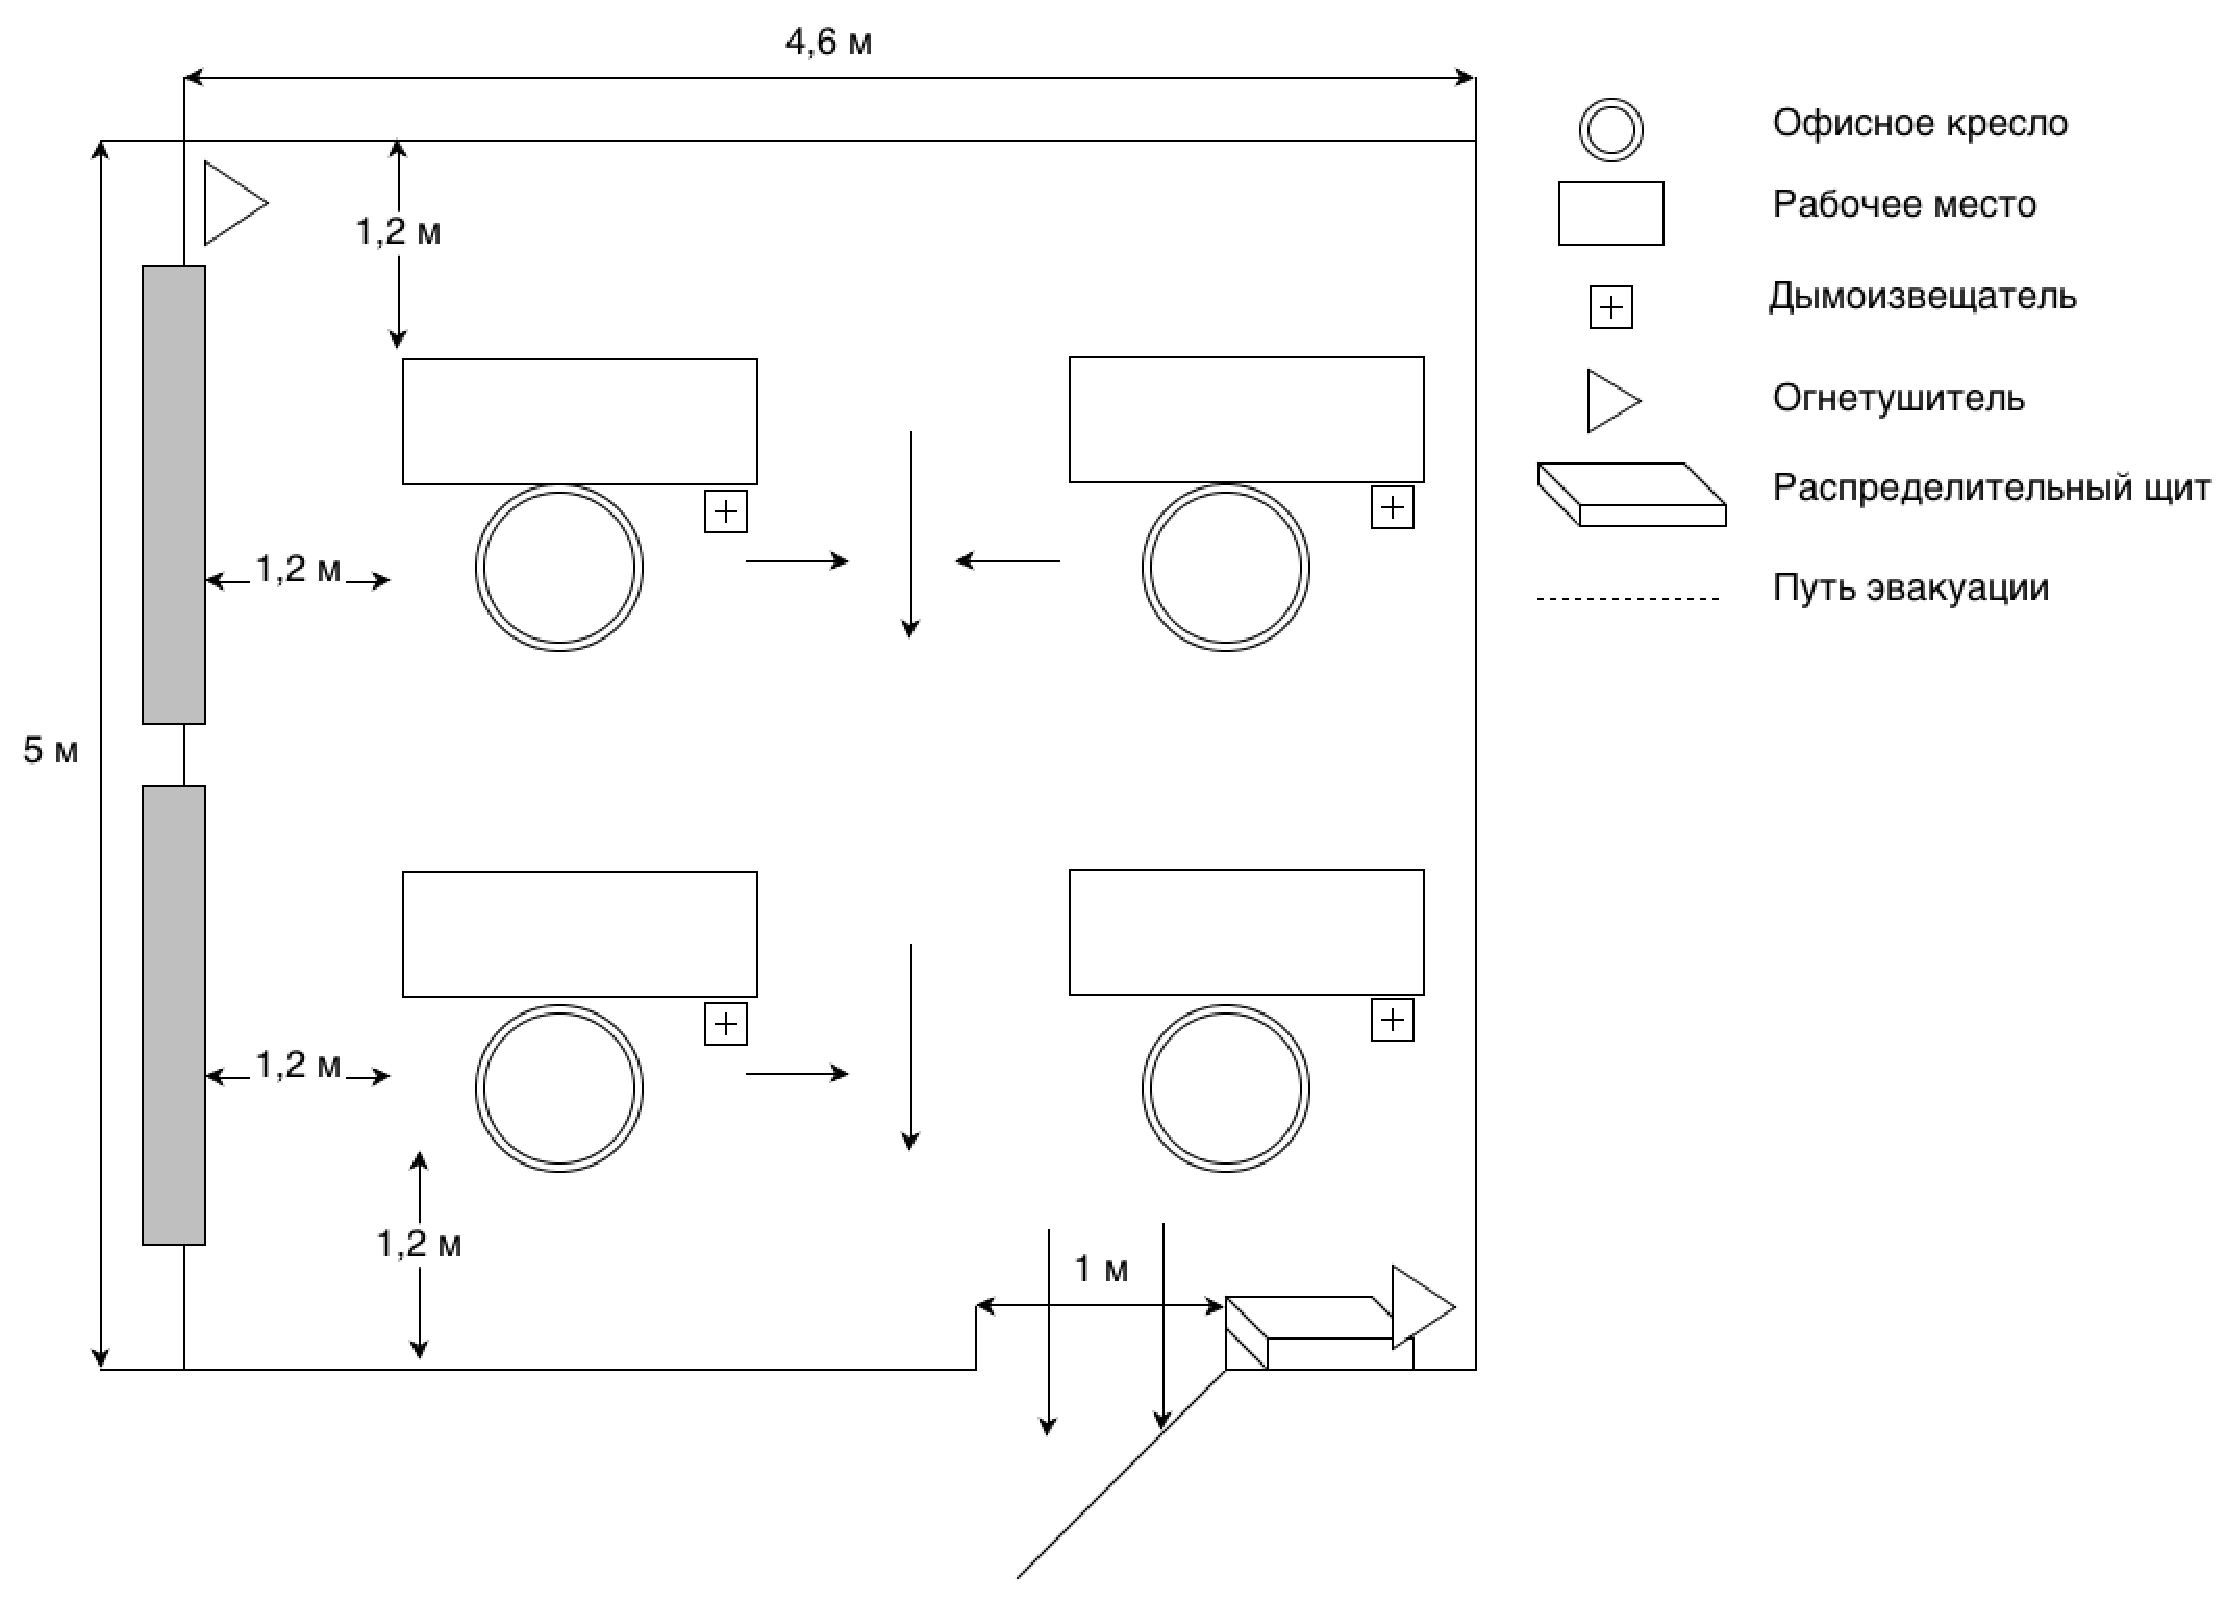
\includegraphics[width=1\textwidth]{graphics/work_places.eps}
    \end{center}
    \caption{Схема размещения рабочих мест в помещении НИЛ}
    \label{fig:work_places}
\end{figure}



\section{Безопасность в чрезвычайных ситуациях}

Защита населения в чрезвычайных ситуациях представляет собой комплекс
взаимосвязанных по месту, времени, цели и ресурсам мероприятий, направленных на
защиту жизни и здоровья людей в любых ЧС.  Указанные мероприятия должны
планироваться и в максимально возможной степени проводиться заблаговременно и на
всей территории страны, охватывая все категории населения.

Объем и содержание мероприятий инженерно-технической защиты населения, правила и
порядок их осуществления устанавливаются в соответствии с требованиями
действующего законодательства и нормативных правовых актов по вопросам защиты
населения и территорий от чрезвычайных ситуаций и от опасностей, возникающих при
ведении военных действий и с учетом экономических, природных и иных особенностей
конкретных территорий, зон, городских и сельских поселений и реальной опасности
для населения в мирное и военное время.

Основными инженерно-техническими мероприятиями по защите населения являются:

\begin{itemize}

    \item укрытие людей в приспособленных для их защиты помещениях
    производственных, общественных и жилых зданий, а также в специальных
    защитных сооружениях;
    
    \item повышение надежности систем жизнеобеспечения (водоснабжение,
    энергопитание, теплофикация и др.) при авариях, катастрофах, стихийных
    бедствиях и в военное время, а также устойчивости жизненно важных объектов
    социального и производственного назначения;
    
    \item выполнение ряда градостроительных требований, позволяющих при
    крупномасштабных ЧС и применении в военных конфликтах современных средств
    поражения уменьшить количество жертв, обеспечить выход населения из
    разрушенных частей города в парки и леса загородной зоны, а также создать
    условия для ввода в пораженную зону аварийно-спасательных сил.

\end{itemize}
    
Основным способом защиты населения от современных военных средств поражения, от
крупномасштабных ЧС, вызванных авариями и катастрофами на химически и
радиационно-опасных объектах, взрывами и пожарами, остается укрытие персонала
предприятий и населения городов в защитных сооружениях.

В соответствии с действующими нормами и правилами по вопросам выполнения
инженерно-технических мероприятий гражданской обороны, а также строительными
нормами и правилами (СНиП) к защитным сооружениям относятся убежища и
противорадиационные укрытия.

Производство, включающее научно-исследовательскую лабораторию, имеет категорию В
пожаровзрвыоопасности, согласно НАПБ Б.03.002-2007. Степень огнестойкости здания
--- II, согласно ДБН В.1.1.7-2002, так как помещение расположено в кирпичном
здании, при строительстве использовались твёрдые несгораемые материалы.

Возможные причины возникновения пожара на рабоем месте или в помещении:

\begin{itemize}

    \item короткое замыкание, сопровождающееся искрением и перегревом элементов
    ПК вследствие чего происходит воспламенение оборудования;

    \item перегрев элементов ПК в следствии высокой нагрузки во время проведения
    атаки;

    \item кабели для подачи электропитания.

\end{itemize}

Согласно ДБН В.2.5.-13-98 в помещении установлено четыре точечных дымовых пожарных
извещателя. В помещении присутствуют два углекислотных огнетушителя ВВК-1,4 из
расчета 1 огнетушитель на 3 ПК, но не менее 1 на помещение, согласно НАПБ
Б.03.001-2204.

Схема эвакуации нанесена на схеме размещения рабочих мест в помещении НИЛ на
рисунке~\ref{fig:work_places}.
